\documentclass[10pt,a4paper]{article}

\usepackage[utf8]{inputenc}
\usepackage[T1]{fontenc}
\usepackage[a4paper,margin=0.75in]{geometry}
\usepackage{tabularx}
\usepackage{array}
\usepackage{booktabs}
\usepackage{enumitem}
\usepackage{graphicx}
\usepackage[hidelinks]{hyperref}

\setlength{\parindent}{0pt}
\setlength{\parskip}{4pt}
\setlength{\tabcolsep}{5pt}
\renewcommand{\arraystretch}{1.1}

\begin{document}

\begin{center}
{\Large \textbf{System Documentation}}\\
\vspace{0.25em}
{\large \textbf{Business Sustainability Management Platform}}\\
\vspace{0.35em}
{\small\itshape Group 9 -- Five Guys}
\end{center}

\vspace{0.35em}
\hrule
\vspace{0.5em}
\small
\textbf{Document Type:} System Documentation Draft\\
\textbf{Filename:} 9\_system\_draft.pdf\\
\textbf{Project Focus:} A web-based ESG and sustainability management platform for multi-store business operations

\vspace{0.5em}
\hrule
\vspace{0.6em}
\normalsize

\section*{Abstract}
This document presents the system documentation for the Business Sustainability Management Platform developed by Group 9. The platform is intended to support practical ESG management in a multi-store business setting through integrated carbon tracking, waste management, sustainability reporting, alert monitoring, and governance-related ESG functions. Instead of relying on separate spreadsheets or isolated reports, the system provides a browser-based workflow that supports structured record keeping, clearer data visibility, and role-sensitive access.

The implemented system combines operational sustainability functions with higher-level governance features. Core modules include dashboard analytics, carbon and waste data recording, sustainability report generation, alert threshold management, supplier ESG assessment, ESG policy management, staff training records, compliance scoring, anomaly detection, user management, and audit logging. The platform also includes supporting functions such as OCR-assisted bill scanning, PDF export, mock fallback strategies for demonstration stability, and multi-role access control for administrators, headquarters managers, regional managers, and store staff.

Technically, the platform is implemented using Flask, Jinja2, Bootstrap, MySQL, and several supporting tools including Flask-Mail and WeasyPrint. In its current form, the system is complete enough to be tested and demonstrated, while still being lightweight enough for browser-based use and academic evaluation.

\section*{1. Introduction}

\subsection*{1.1 Project Background}
Environmental, Social, and Governance (ESG) concerns have become more important in business management, especially for organisations that operate across multiple physical locations and need more consistent sustainability oversight. In restaurant and coffee-shop style businesses, day-to-day sustainability work often includes repetitive operational tasks such as recording energy use, tracking waste generation, monitoring recycling performance, and preparing summary reports for management review. In many cases, however, these tasks are still handled through separate spreadsheets, manually prepared documents, or informal communication between branches. This makes long-term monitoring harder and can also reduce the transparency of sustainability claims.

The Business Sustainability Management Platform was developed to respond to this problem in a practical way. The project focuses on building a web-based platform that can bring sustainability-related operational data and governance functions into one interface. By integrating data collection, analytics, reporting, alerts, and ESG management, the system aims to improve traceability, consistency, and visibility for sustainability work across multiple stores.

\subsection*{1.2 Problem Statement}
Before this platform was developed, sustainability-related activities in the target business scenario were difficult to monitor in a consistent and structured way. Carbon records, waste records, and reporting outputs could be created, but they were not easy to standardise across different stores. Management therefore lacked an efficient way to compare branch performance, detect unusual data patterns, monitor reporting coverage, or evaluate suppliers from an ESG perspective. At the same time, different users needed different permissions, which meant that a realistic solution required not only data-entry pages but also a clear access-control model.

The system was therefore designed to address three linked problems. First, it needed to provide a reliable operational layer for recording carbon and waste data. Second, it needed to turn these data into useful management outputs such as dashboards, reports, and alerts. Third, it needed to extend beyond operational monitoring into governance-oriented ESG management through supplier assessment, policy management, compliance scoring, and audit support.

\subsection*{1.3 Project Objectives}
The main objective of the project is to create a practical ESG management platform that supports both sustainability operations and management decision-making. To achieve this objective, the project was designed around several concrete goals:

\begin{itemize}[leftmargin=1.4em,itemsep=2pt,topsep=2pt]
    \item provide structured carbon and waste tracking workflows for different business roles;
    \item support dashboard-based data visualisation and summary analysis;
    \item enable sustainability report generation and PDF export;
    \item provide alert and notification functions for management monitoring;
    \item integrate ESG governance features such as supplier assessment and policy management;
    \item support administrative and assurance functions including compliance scoring, anomaly detection, user management, and audit logging.
\end{itemize}

\subsection*{1.4 Project Planning and Scope Evolution}
The project began with a smaller set of core sustainability management functions focused on carbon tracking, waste management, dashboard review, and reporting support. As development progressed, the system scope changed through iterative refinement and practical implementation decisions. This did not replace the original direction of the project. Instead, it gradually expanded the platform into a more complete ESG management system by adding governance and monitoring features that became more relevant during development.

As a result, the current version of the platform goes beyond basic operational record keeping. It now includes supplier ESG scorecard assessment, ESG policy management, compliance evaluation, anomaly detection, user administration, audit logging, OCR-assisted input support, and alert-based monitoring. The final system reflects both the original sustainability-management direction and the later integration of governance, assurance, and decision-support functions.

\subsection*{1.5 Target Users}
The platform is designed for four main user roles: administrators, headquarters managers, regional managers, and store staff. These roles differ in both their responsibilities and their access scope. Administrators and headquarters managers can oversee company-wide data and configuration. Regional managers focus on the stores within their region. Store staff primarily create and manage operational records for their own store. This role distinction shaped both the backend access-control logic and the frontend page visibility of the final system.

\section*{2. Technical Implementation}

\subsection*{2.1 System Architecture and Technology Stack}
The platform follows a web-based client-server architecture in which the presentation layer, application layer, and data layer are separated while still remaining lightweight enough for semester delivery. The backend is implemented with Flask and organised through modular blueprints so that each business area, such as carbon tracking, waste management, reporting, alerts, ESG management, and administration, can be maintained as a relatively independent functional unit. This modular structure improves readability, simplifies route organisation, and makes later extension easier when new features are introduced.

\begin{figure}[h]
\centering
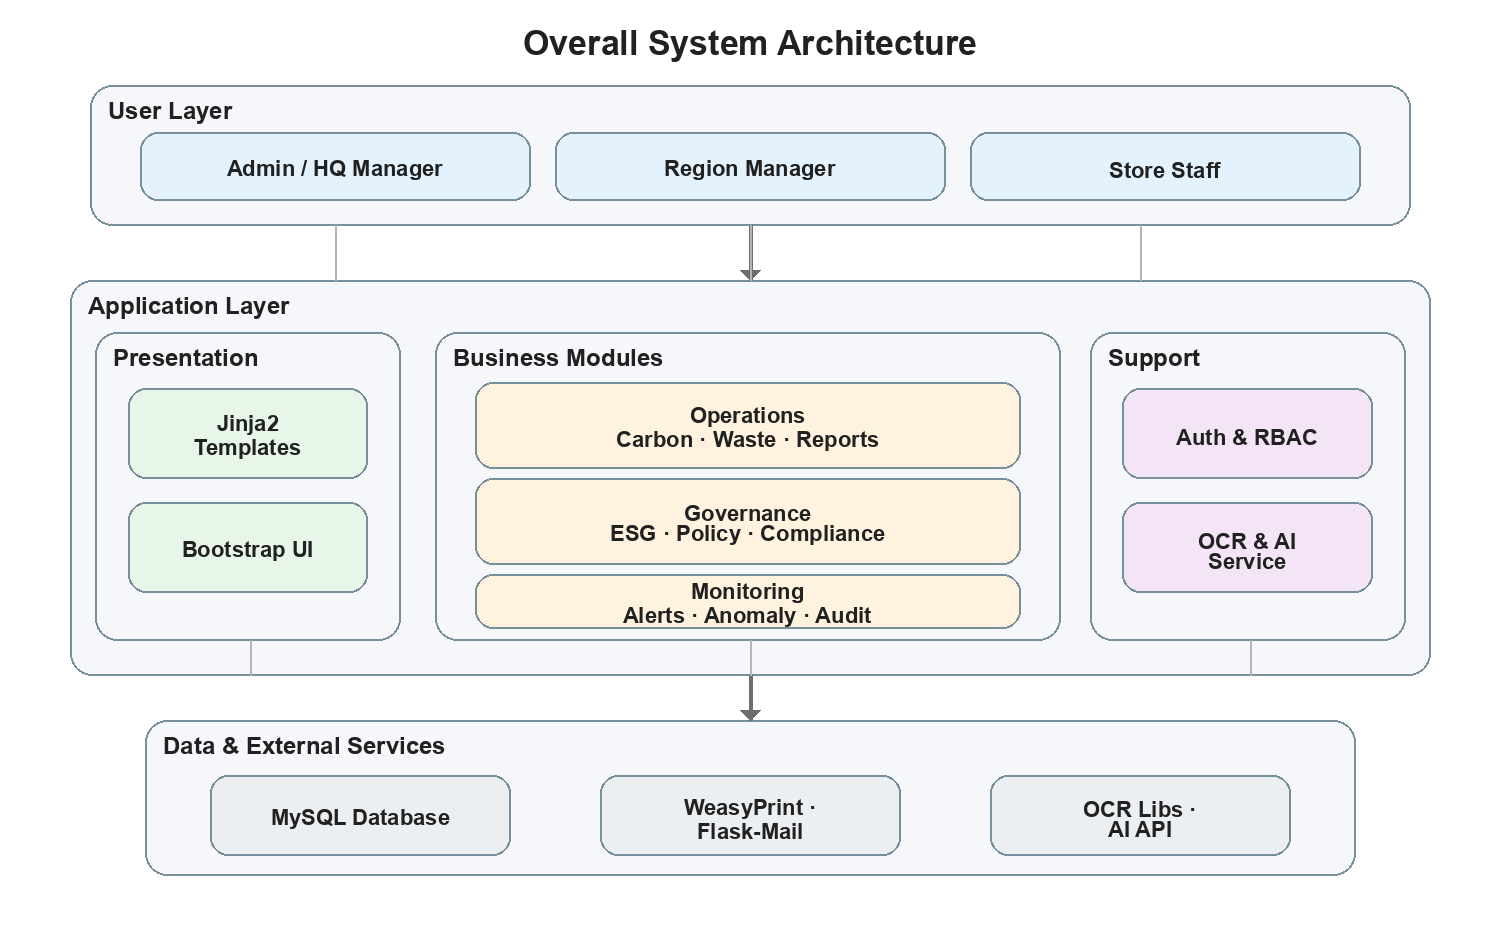
\includegraphics[width=0.92\linewidth]{figures/system_architecture_compact.png}
\caption{Overall System Architecture of the Business Sustainability Management Platform}
\end{figure}

\begin{figure}[h]
\centering
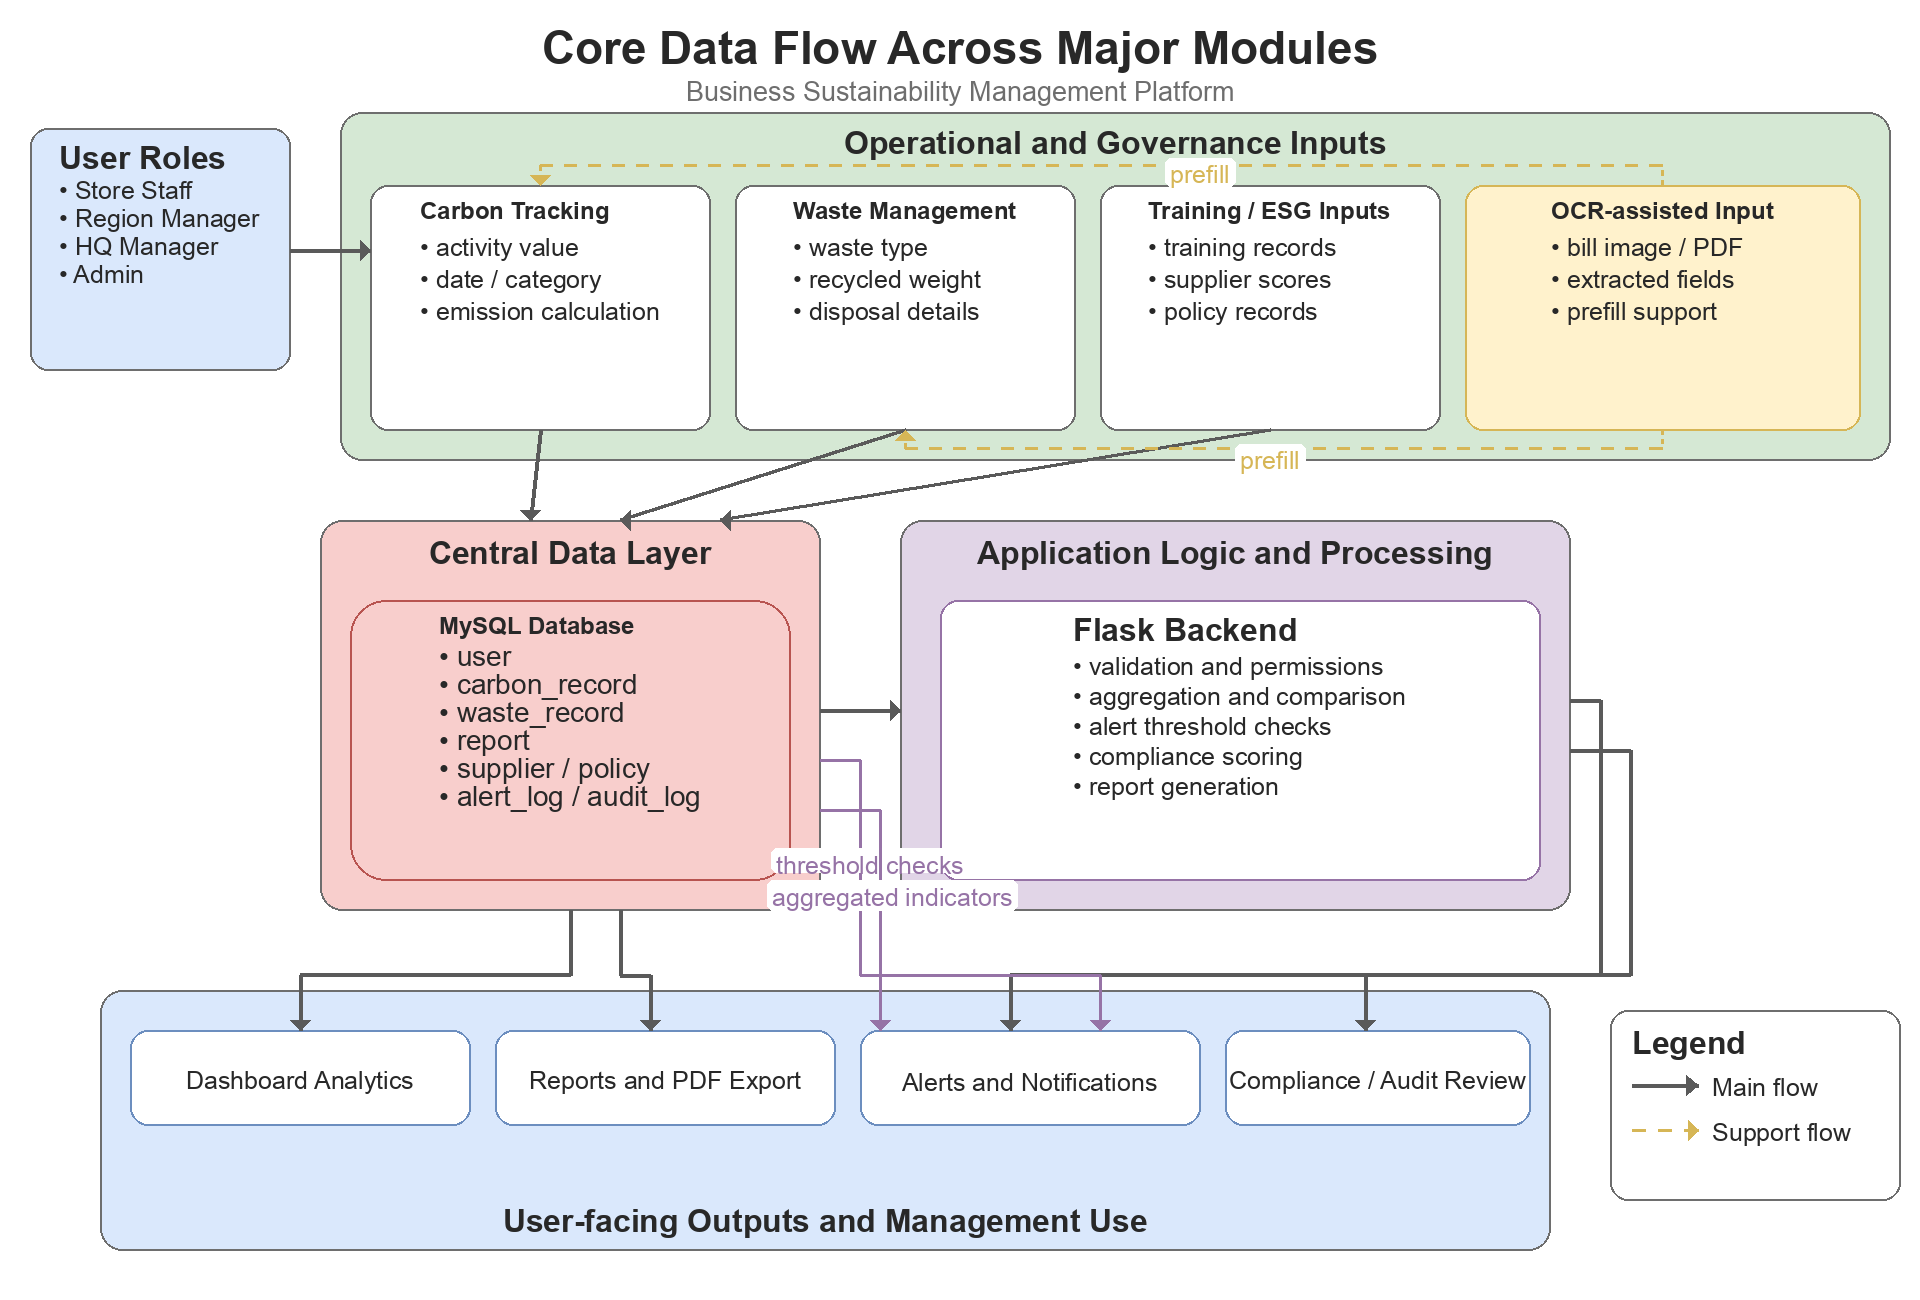
\includegraphics[width=0.95\linewidth]{figures/system_core_data_flow.png}
\caption{Core Data Flow Across Major Modules}
\end{figure}

On the frontend side, the project uses Jinja2 templates combined with Bootstrap to provide a browser-based interface with a consistent layout, reusable interaction patterns, and role-sensitive navigation. This approach suited the project because it allowed us to combine server-rendered pages with lightweight dynamic behaviour without adding an unnecessary single-page-application layer. Shared templates provide consistent headers, sidebars, and visual structure across modules, while module-specific pages focus on tables, forms, filters, charts, and management interactions.

MySQL is used as the persistent data layer for operational records, governance data, user information, alert logs, report content, and audit history. This choice supports structured querying, aggregation, and longer-term storage across several related modules. It is important because the platform does not only record isolated entries; it also reuses those records in comparisons, dashboards, reporting, compliance scoring, and anomaly detection. Supporting utilities extend this architecture in more specific ways. Flask-Mail is used for notification support, WeasyPrint is used for PDF report generation, and optional OCR-related libraries support scanned bill extraction when the environment permits. Together, these choices create a system that is not overly complex technically, but still broad in functionality.

\begin{table}[h]
\centering
\scriptsize
\begin{tabularx}{\linewidth}{@{}p{0.24\linewidth}p{0.10\linewidth}X@{}}
\toprule
\textbf{Table / View} & \textbf{Category} & \textbf{Role in the System} \\
\midrule
company, region, store & Organisation & Define the three-level hierarchy (HQ $\rightarrow$ region $\rightarrow$ store) used for data isolation and scope-based access control \\
user & Identity & Store credentials, role (admin / hq\_manager / region\_manager / store\_staff), and organisational scope for session-based authentication \\
emission\_factor & Reference & Pre-seeded lookup of emission coefficients by category and sub-type, used to convert activity values into carbon kg during record creation \\
carbon\_record & Operations & Record-level carbon data including activity value, calculated emissions, category, store, and date; feeds dashboards, reports, alerts, and comparisons \\
waste\_category & Reference & Enumeration of waste types with recyclability flags; referenced by waste records for classification \\
waste\_record & Operations & Record-level waste data including weights, disposal method, and store; contributes to recycling analysis, compliance, and reporting \\
report & Reporting & Persisted sustainability report with aggregated carbon and waste summaries, SDG indicators, optional AI commentary, and PDF export support \\
sdg\_goal, company\_sdg & Governance & UN SDG reference data and per-company alignment tracking with target values and progress percentages \\
alert\_threshold & Monitoring & Configurable metric thresholds at company / region / store level for waste recycling rate, carbon MoM growth, and daily waste weight \\
alert\_log & Monitoring & Triggered alert records with metric snapshots, read-state management, and optional email notification tracking \\
audit\_log & Audit & Immutable log of user actions (login, create, update, delete, export) for traceability and compliance review \\
supplier & Governance & Supplier records with a 16-indicator ESG scorecard across carbon, waste, ethics, and reporting dimensions; rule-based scoring \\
esg\_policy & Governance & Internal ESG policy documents with versioning, status lifecycle (draft / active / archived), and category tagging \\
\midrule
v\_carbon\_monthly\_summary, v\_waste\_monthly\_*  & View & Monthly aggregated carbon and waste summaries by store; used for dashboard charts and MoM trend comparisons \\
v\_store\_carbon\_summary, v\_store\_waste\_summary & View & Store-level monthly totals used internally for alert threshold evaluation (MoM growth and recycling rate) \\
\bottomrule
\end{tabularx}
\caption{Key Database Entities and Their Roles}
\end{table}

At a high level, users interact with the system through browser-based pages and forms, submit or review data according to their role, and trigger backend logic that validates, stores, and transforms those data into management outputs. Submitted records then become part of a wider internal data flow: carbon and waste data feed dashboards and reports, alerts are triggered by thresholds linked to new records, compliance scoring aggregates indicators across modules, and governance pages draw on structured policy and supplier information. In this way, the architecture supports both day-to-day operational use and higher-level ESG management workflows within one platform.

\subsection*{2.2 Authentication and Role-Based Access Control}
The system uses username-and-password authentication with server-side session management. After successful login, the backend stores key identity and scope information in the session, including the current user's role, company, region, and store context. This design fits a server-rendered Flask application because it keeps access control logic close to the business routes and avoids exposing sensitive authorisation state on the client side.

Authentication alone is not sufficient for this platform because different users require access to different stores, different forms, and different management pages. For that reason, role-based access control is implemented as a core design principle rather than as something added later. Administrators and headquarters managers can access company-wide data and configuration, regional managers are limited to stores in their assigned region, and store staff are restricted to their own store and a narrower set of operational actions. This distinction affects not only API endpoints but also visible navigation items, editable records, and management permissions.

The system also applies more granular restrictions within modules. For example, store staff can create and manage operational records but are subject to tighter edit and delete windows, while higher-level management roles can configure alerts, manage users, access compliance views, and use governance-focused features such as supplier ESG assessment and policy management. This multi-layered approach makes the system more realistic because real organisations do not only distinguish between ``logged in'' and ``not logged in'' users; they also need to reflect reporting hierarchies and operational accountability. As a result, access control in this platform works as a structural feature of the overall system rather than only as a narrow security add-on.

\begin{table}[h]
\centering
\scriptsize
\begin{tabularx}{\linewidth}{@{}p{0.14\linewidth}p{0.15\linewidth}p{0.14\linewidth}p{0.11\linewidth}p{0.12\linewidth}X@{}}
\toprule
\textbf{Role} & \textbf{Scope} & \textbf{Carbon/Waste} & \textbf{Reports} & \textbf{Alerts} & \textbf{Key Management Functions} \\
\midrule
Admin & Company-wide & Full CRUD & Full & Config + review & Users, audit, compliance, anomaly, ESG management \\
HQ Manager & Company-wide & Full CRUD & Full & Config + review & Compliance, anomaly, ESG management, company users \\
Region Manager & Assigned region & Regional access & Regional & Review only & Compliance, anomaly, dashboard drilldown \\
Store Staff & Own store only & Own-store with time limits & Limited use & No config & No admin or governance configuration \\
\bottomrule
\end{tabularx}
\caption{Role-Based Access Scope and Functional Permissions}
\end{table}

\subsection*{2.3 Dashboard and Data Visualisation}
The dashboard module transforms recorded operational data into summary indicators and management-oriented visualisations. It provides an overview of total carbon emissions, total waste, recycling performance, and report volume, while also supporting chart-based review of carbon trends, waste composition, and category-level breakdowns. Drilldown support enables users to move from aggregated company or regional indicators to more specific store-level views.

An additional analytical layer connects the dashboard to SDG 12 related indicators, including waste recovery, carbon efficiency, reporting coverage, and store data coverage. This makes the dashboard not only a display page but also a compact decision-support surface for sustainability oversight.

\subsection*{2.4 Carbon Tracking Module}
The carbon tracking module supports the structured recording of carbon-related operational data and forms one of the most important operational foundations of the platform. In practice, this module is intended to capture recurring store-level activities that can be associated with carbon impact, such as electricity use or other emissions-relevant activities. Users enter activity values, dates, categories, and related contextual information, while the backend applies validation and calculation logic before committing the record to the database.

An important implementation detail is the use of emission-factor-based calculation. Instead of storing only a manually entered carbon total, the system links activity data with an emission context and calculates the resulting carbon value automatically. This improves consistency and reduces the risk of arbitrary reporting. It also makes the module more reusable, because once the raw operational input has been recorded, the resulting carbon totals can be reused across several other parts of the platform, including dashboards, reports, comparisons, and compliance-related calculations.

The module also contains operational controls that make it more realistic than a basic data-entry form. Users can list, add, edit, and delete records, but these actions are constrained by both role scope and time-based business rules. In particular, store staff are subject to a limited modification window, which reduces the likelihood of uncontrolled retroactive editing while still allowing reasonable correction of recent mistakes. This mirrors the practical idea that store-level data should be editable when first recorded but should not remain indefinitely open to change.

In addition to recording data, the module supports management-oriented analysis. Comparison functions enable month-on-month review and store-versus-region benchmarking so that managers can identify abnormal increases or performance differences between locations. Export support further improves practical usability by allowing data extraction beyond the live application view. The module is also strengthened by OCR-assisted input support, which helps prefill operational data from scanned bills or similar documents. For these reasons, the carbon module is not only a record-keeping page but a structured workflow that connects calculation, control, and analysis.

\subsection*{2.5 Waste Management Module}
The waste management module provides a structured way to record, review, and analyse waste-related operational data. It captures information such as waste category, total waste weight, recycled quantity, source type, disposal method, disposal unit, notes, dates, and store linkage. These fields make the module more informative than a simple waste total, because they allow users and managers to understand not only how much waste was produced but also what kind of waste was generated and how it was handled.

Validation is particularly important in this module because waste data are often vulnerable to inconsistent manual entry. The backend therefore enforces required fields, sensible numeric constraints, and practical business rules such as ensuring that recycled weight does not exceed total recorded waste. Store scope restrictions are also applied so that users only interact with records within their permitted organisational boundary. Together, these rules help preserve data quality before the information is reused elsewhere in the system.

Like the carbon module, waste management supports record listing, creation, editing, and deletion. It also applies time-based restrictions for lower-permission users so that ordinary operational records remain manageable but not indefinitely mutable. This reflects a design principle used throughout the platform: operational flexibility is allowed, but long-term traceability is prioritised once data have become part of organisational monitoring.

The management value of this module extends beyond the raw record table. Waste data contribute to recycling analysis, trend comparison, dashboard summaries, report content, and compliance-related indicators. Comparison support enables users to review current performance against previous periods or wider organisational averages, while export support improves the practical portability of the data. Because waste handling is closely connected with responsible consumption and recovery performance, this module also plays a significant role in the system's connection to broader ESG and SDG-oriented reporting.

\subsection*{2.6 Sustainability Reporting Module}
The sustainability reporting module is one of the clearest examples of how the platform transforms operational records into management-ready outputs. Rather than requiring users to manually rewrite carbon and waste statistics into separate documents, the system aggregates data within a selected time range and generates structured report content directly from stored records. This allows reporting to remain connected to the same data foundation used elsewhere in the application and reduces duplication of work.

From an implementation perspective, the module performs several linked tasks. It accepts a reporting period, queries the relevant carbon and waste data, derives summary values, and then stores the resulting report as a persistent record in the database. This means that a report in the platform is not just a temporary generated page; it becomes a reusable artefact that can later be listed, viewed in detail, exported, or deleted. This approach improves traceability because reporting history can be examined over time instead of being regenerated from scratch each time.

PDF export is a major part of this module. The system first renders report content through a Jinja2-based HTML structure and then uses WeasyPrint to produce a downloadable PDF. This design fits the wider architecture well because it reuses templating logic already present in the web layer while still generating a formal document output suitable for submission, review, or demonstration. The report content is also connected with SDG 12-related indicators so that the final output contains not only raw totals but also more interpretive sustainability information.

Another important extension is AI-assisted report commentary. The system supports a real external API pathway for generating narrative ESG comments while also preserving a mock fallback path for development and testing contexts. This fallback strategy is significant because it allows the report module to remain demonstrable even when external services are unavailable. In the final system, the reporting module therefore operates as a bridge between stored operational data, analytical interpretation, formal PDF export, and optional AI-enhanced commentary.

\begin{figure}[h]
\centering
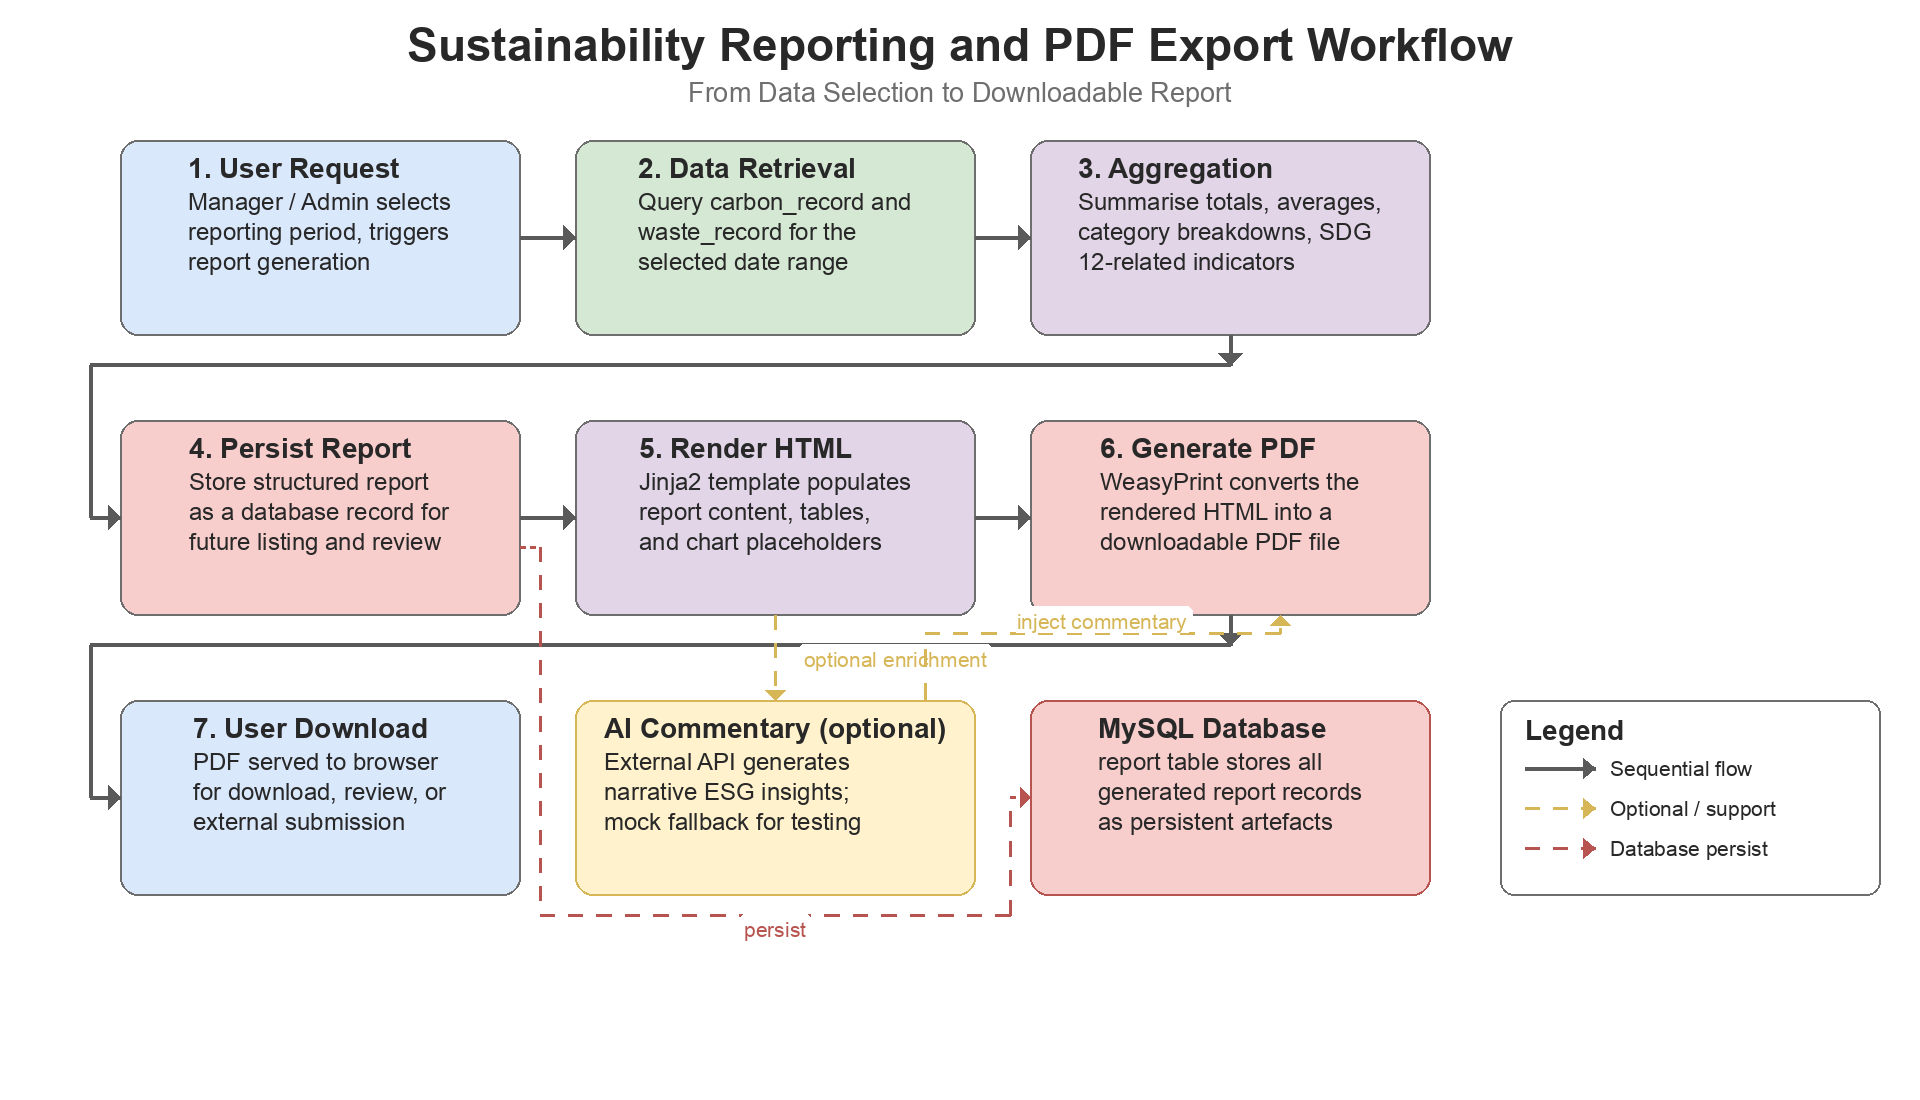
\includegraphics[width=\textwidth]{figures/report_workflow.png}
\caption{Sustainability Reporting and PDF Export Workflow}
\end{figure}

\subsection*{2.7 Alerts and Notification Mechanism}
The alert subsystem provides threshold-based monitoring for sustainability performance. Users with appropriate permissions can define thresholds for selected metrics at company, region, or store level. When new operational data are processed, relevant alert logic can be triggered and recorded for later review.

The module supports alert logs, unread-count indicators, and read-state management, making it suitable for ongoing managerial monitoring rather than one-time reporting only. Email-based notification support is also integrated through Flask-Mail, while fallback behaviour helps preserve usability in test or demo environments where full mail configuration may not be available.

\subsection*{2.8 ESG Management Module}
The ESG Management section combines supplier assessment and ESG policy management under a unified interface. This reflects the fact that ESG management in practice involves both operational evaluation of partners and the maintenance of governance rules within the organisation. Structurally, placing these functions together also improves the clarity of the system because it distinguishes governance-oriented ESG work from day-to-day operational record entry.

This part of the system is particularly important because it shows that the platform is not limited to measuring internal store activity. It also supports broader organisational responsibilities such as evaluating external partners and maintaining internal ESG policy records. In other words, this module extends the system from environmental operations into governance-oriented sustainability management.

\subsubsection*{2.8.1 Supplier ESG Assessment}
The supplier module manages supplier records while also evaluating them through a rule-based ESG scorecard. The current model uses four dimensions---carbon, waste, ethics, and reporting---and each dimension contains four sub-indicators scored as 0, 50, or 100. Weighted aggregation is then used to calculate both dimension-level scores and an overall grade. This design was chosen deliberately. A simple manual score field would be too opaque, while a data-hungry black-box model would not be realistic for the project context. The implemented scorecard therefore offers a middle ground: it is structured, explainable, and practical.

The use of 0, 50, and 100 as discrete scoring values makes the model easier to interpret during data entry and later review. It encourages users to think in terms of whether a supplier does not meet, partially meets, or clearly meets a given ESG-related expectation. Because the model is rule-based, score changes can be explained directly by the selected sub-indicators rather than hidden behind inaccessible logic. This is especially useful for academic demonstration, where transparency and justification are more important than claiming unrealistic predictive sophistication.

\begin{table}[h]
\centering
\scriptsize
\begin{tabularx}{\linewidth}{@{}p{0.15\linewidth}p{0.40\linewidth}p{0.15\linewidth}X@{}}
\toprule
\textbf{Dimension} & \textbf{Example Sub-indicators} & \textbf{Score Options} & \textbf{Purpose} \\
\midrule
Carbon & Disclosure, reduction target, carbon monitoring, supporting evidence & 0 / 50 / 100 & Evaluates whether the supplier tracks and improves carbon-related performance \\
Waste & Waste reduction, recycling practice, disposal control, waste reporting & 0 / 50 / 100 & Captures resource-efficiency and waste-handling responsibility \\
Ethics & Labour practice, compliance awareness, traceability, ethical policy support & 0 / 50 / 100 & Reflects social and governance expectations in supplier behaviour \\
Reporting & ESG disclosure, consistency, completeness, review readiness & 0 / 50 / 100 & Measures the supplier's reporting transparency and management maturity \\
\bottomrule
\end{tabularx}
\caption{Structure of the Supplier ESG Scorecard}
\end{table}

From a workflow perspective, the supplier module supports adding, editing, listing, and deleting supplier records, while automatically recalculating ESG scores whenever data are submitted. This removes dependence on manually entered total scores and ensures that the overall grade remains aligned with the selected sub-indicator values. The result is a supplier assessment workflow that is operationally manageable for users but still rigorous enough to represent a real governance-oriented evaluation mechanism.

\subsubsection*{2.8.2 ESG Policy Management}
The ESG policy module manages internal policy records such as policy category, version, status, effective date, and content. These records are presented within the same ESG Management area as supplier assessment, which creates a stronger governance-oriented workflow. In practical terms, this allows the system to represent both ESG evaluation and ESG policy maintenance within one management space.

Although the policy module is structurally simpler than supplier scoring, it is important for completeness. ESG management in a realistic organisation does not only involve measuring outcomes; it also involves maintaining policy documents, version control, implementation status, and effective dates. By including these fields in the system, the platform supports a clearer connection between governance rules and operational sustainability practices.

\subsection*{2.9 Training and Compliance Evaluation}
Training and compliance functions extend the system from operational data collection into organisational improvement and assurance. The training module stores sustainability-related training records, course types, completion data, scores, and summary statistics. These records help represent staff capability development as part of ESG management rather than as a disconnected administrative activity. In other words, the system recognises that sustainability performance does not depend only on recorded outcomes, but also on whether staff are being prepared to carry out related practices consistently.

The compliance score module builds on this wider perspective by aggregating multiple ESG-relevant dimensions, including carbon management, waste and recycling, staff training, reporting frequency, and alert resolution. This design is useful because it combines operational and managerial signals rather than relying on a single metric. For example, an organisation might record waste data consistently but perform poorly in training coverage or alert handling. A broader compliance score therefore provides a more balanced summary of the organisation's ESG readiness and discipline.

\begin{table}[h]
\centering
\scriptsize
\begin{tabularx}{\linewidth}{@{}p{0.22\linewidth}p{0.26\linewidth}X@{}}
\toprule
\textbf{Dimension} & \textbf{What It Measures} & \textbf{Main Data Source} \\
\midrule
Carbon Management & Consistency and quality of carbon-related operational records & Carbon tracking records and comparisons \\
Waste and Recycling & Waste handling quality, recycling performance, and recovery-related behaviour & Waste management records and recovery metrics \\
Staff Training & Participation, completion, and coverage of sustainability-related training activity & Training records and summary statistics \\
Reporting Frequency & Whether sustainability reporting is being produced regularly and in usable form & Stored report records and reporting history \\
Alert Resolution & Whether monitored issues are noticed, logged, and followed through at management level & Alert thresholds, alert logs, and review status \\
\bottomrule
\end{tabularx}
\caption{Dimensions Used in ESG Compliance Evaluation}
\end{table}

By calculating a weighted total score and final grade, the platform presents a compact but meaningful summary of broader ESG performance that goes beyond individual operational records. This is particularly valuable for management review, because it converts distributed activity across multiple modules into a form that can be read quickly and compared more easily over time. In this sense, compliance evaluation acts as a synthesis layer that connects operational data quality, process discipline, and governance-oriented performance.

\subsection*{2.10 Advanced Management and Support Functions}
Several additional modules increase the completeness and practical value of the platform. Anomaly detection applies statistical and rule-based checks to carbon and waste records in order to highlight abnormal data patterns. User management enables higher-permission users to create, update, and remove accounts, assign roles, and reset passwords. Audit logging records major system actions and improves traceability for management and review.

The platform also supports OCR-assisted bill scanning. Uploaded bill images or PDFs can be processed to extract useful fields such as category, activity value, date, invoice number, and supplier name, which can then help prefill sustainability data entry workflows. This feature improves usability while also demonstrating an advanced input-assistance pathway.

\subsection*{2.11 Database, Migration, and Deployment Support}
The platform depends on a structured MySQL schema that stores user, operational, reporting, governance, and monitoring data. Because the system evolved throughout the semester, migration support became an important part of implementation. Migration scripts are used to update schema structure in an incremental and repeatable way, including support for newly introduced ESG scorecard fields and related data changes.

The project also uses fallback strategies to improve robustness in evaluation settings. Mock data and fallback execution paths are available for selected modules such as supplier records, policy content, AI commentary, OCR input, and email notification. This helps maintain functional demonstrations even when external services or optional dependencies are unavailable.

\section*{3. Use of Generative AI}
Generative AI tools were used during this project as supporting assistants rather than as something that could design or build the whole system for us. In our team, they were mainly useful for speeding up medium-sized tasks such as rewriting documentation drafts, suggesting alternative code structures, summarising route behaviour, adjusting UI wording, and giving possible debugging directions when we ran into errors. AI was also helpful when we needed to turn rough ideas into clearer technical descriptions, especially for documentation sections, figure explanations, and cross-module workflow summaries.

At the same time, we did not treat AI output as something we could trust directly. This was especially important in our project because the platform contains many connected modules, role-based permissions, and business rules that are easy to describe incorrectly if the prompt is too general. For example, an AI tool could produce a convincing explanation of which user roles can access a page, how a score is calculated, or what a route stores in the database, while still being wrong in important details. In a Flask project with many blueprints, templates, and permission boundaries, even a small hallucination could lead to inaccurate documentation or a bad implementation decision.

In practice, our use of AI was mainly in four areas. First, it supported coding productivity by suggesting possible implementations, refactoring ideas, or bug-fix directions for selected modules. Second, it helped with debugging by interpreting error messages and suggesting likely causes or missing dependencies. Third, it was useful in documentation work, where it helped us improve wording, shorten repetitive explanations, and reorganise technical content into a clearer academic structure. Fourth, it helped with design communication by turning partially formed ideas into clearer descriptions that we could then compare with the actual codebase.

Even with these benefits, we found several limitations. AI-generated code can look correct at first sight while still not matching the real project architecture. Some suggestions ignored the actual database schema, used the wrong variable names, mentioned packages that were not available, or described features that we had not really implemented. The same problem appeared in writing tasks. AI could produce fluent paragraphs that sounded formal, but sometimes they made a feature sound more mature than it really was, or blurred the difference between an implemented function and a possible future extension. For system documentation, this kind of mistake is a serious problem because the document should describe the real system, not an ideal version of it.

Because of this, we checked AI-assisted output manually before keeping it. Code suggestions were compared with the existing Flask routes, template behaviour, schema design, and current module responsibilities. Documentation text was checked against actual pages, backend permission restrictions, and known business logic so that we did not accidentally invent permissions, workflows, or feature boundaries. When AI suggested packages, commands, or LaTeX changes, we also verified them through local compilation or direct inspection instead of accepting them only because they sounded reasonable. So although AI helped us move faster, final acceptance still depended on normal software engineering judgement.

This also changed how our team thought about using AI. Instead of asking it to ``build the system'', the more reliable way was to use it as a reviewer, writing assistant, and idea-expansion tool. It worked best when one of us already understood the target file, module, or documentation section well enough to judge whether the suggestion actually matched the project. It worked much worse when the prompt was too open-ended or did not provide enough project context, because that made hallucination more likely. From our experience, the usefulness of AI depended a lot on how specific the prompt was and how carefully the result was checked afterwards.

Overall, generative AI did improve our development speed and documentation efficiency, but it did not reduce the need for human judgement. If anything, it made checking more important, because plausible-looking mistakes were easier to produce. For that reason, our team treated AI as a productivity tool rather than a replacement for technical responsibility. This was consistent with the wider goal of the project: to deliver a system that is functional, demonstrable, and honestly described. In that sense, AI was genuinely helpful in this project, but only when we used it with enough context and checked the results carefully.

\section*{4. Groupwork}
Our project followed a work-package structure, so each member had a main area to focus on, while still helping with integration and later revisions across the system. This worked reasonably well for our team because it gave everyone clear responsibilities without making the work completely separate. As the project developed, several modules became more connected than we expected at the beginning, especially around ESG management, reporting, compliance, and integration. Because of that, the final contribution pattern was not only based on the original work-package plan, but also on the adjustments we made during implementation.

\subsection*{4.1 Yao Tianren}
Yao Tianren was mainly responsible for WP1, which covered requirements analysis and overall system design. His main contribution was to help define the scope of the project and turn broad sustainability goals into a system structure that could realistically be implemented within one semester. This included analysing the likely needs of business users, identifying key scenarios for carbon tracking, waste management, and sustainability reporting, and helping shape the project into a multi-role ESG management platform rather than just a few separate record pages.

Besides the early planning work, he also contributed to the technical direction and the overall modular structure of the platform. His work included system architecture planning, functional decomposition, database structure planning, and low-fidelity design preparation. These early design choices influenced later modules such as ESG policy management, supplier assessment, and compliance-related workflows. He also took part in reviewing design artefacts and discussing revisions so that later implementation still matched the original aims of the project.

\subsection*{4.2 Liu Haopu}
Liu Haopu was mainly responsible for WP2 and WP6, covering backend development as well as project delivery and final documentation. His main contribution was building the backend foundation of the platform, including database instance preparation, schema construction, API design, validation logic, and business-rule handling across the main functional modules. This included account management, carbon and waste workflows, sustainability reporting, alert processing, ESG management, and other core backend services.

His work also extended into later-stage modules that became important in the final version of the platform, such as report generation support, PDF export integration, supplier ESG scorecard logic, policy-related backend support, and migration handling for an evolving database structure. In the final delivery stage, he also worked on system documentation, user-facing setup guidance, testing account preparation, deployment-related tasks, and presentation materials. This made his role closely connected with both implementation and final handover.

\subsection*{4.3 Li Sihang}
Li Sihang was mainly responsible for WP3, which focused on the frontend foundation of the system. His main task was to establish the structural base of the interface layer so that later business modules could be developed in a more consistent way. This included frontend framework setup, page organisation, routing-related coordination in the Flask/Jinja environment, reusable UI component preparation, request integration patterns, and general interface consistency.

He also contributed to role-sensitive frontend behaviour and the shared interaction structure of the system, including navigation layout, shared forms, modal-based interaction patterns, and consistent visual styling. These parts were important because the system supports several user roles with different permissions and visible modules. By building a stable and reusable frontend foundation, he made it easier to integrate later pages such as ESG management, compliance review, and administrative features without major redesign of the shared UI.

\subsection*{4.4 You Haoyang}
You Haoyang was mainly responsible for WP4, which focused on the implementation of core business-facing frontend modules. His contribution was mainly to turn business requirements into user-facing workflows across the main sustainability functions of the platform. This included carbon-tracking pages, waste-management interfaces, reporting-related interaction, and the visual presentation of data through dashboard components and page-level integration.

His work also supported the interactive quality of the system by improving the usability of forms, tables, visual summaries, and role-relevant workflows. As the project developed, this role also extended to the integration of additional operational interfaces connected with report generation, ESG management views, and other business-oriented pages. Through this work, the frontend became more than a set of static pages and moved closer to a coherent interface for daily sustainability management and management review.

\subsection*{4.5 Lu Yuan}
Lu Yuan was mainly responsible for WP5, which focused on system integration, testing, and deployment-oriented refinement. His main task was to connect the database, backend logic, frontend pages, and business workflows into a usable end-to-end platform. This included identifying module interaction problems, supporting compatibility and integration checks, and improving the overall stability of the system as features were brought together.

This contribution became especially important in the later stages of development, when the project expanded to include compliance scoring, anomaly detection, alert review, audit support, and other management-oriented functions. Integration and testing helped make sure these modules were not treated as separate experiments, but as parts of one coherent system. In addition, his role also covered deployment-oriented testing, performance-related refinement, and support for final validation in an environment suitable for demonstration and remote review.

\section*{5. Conclusion}
The Business Sustainability Management Platform has developed into a much more complete system than a simple sustainability data-entry prototype. In its current form, it supports operational record management, role-based access control, dashboard analytics, report generation, alert monitoring, ESG governance workflows, training support, compliance evaluation, anomaly detection, user administration, and audit tracking. Taken together, these functions allow the platform to work both as an operational sustainability tool and as a broader ESG management environment.

One of the main strengths of the implemented system is that it combines everyday business workflows with broader governance and assurance functions. Carbon tracking and waste management provide the main operational data foundation of the platform, while reporting, alerting, compliance scoring, supplier assessment, and policy management extend these records into more meaningful management processes. Additional support functions such as PDF export, OCR-assisted input, audit logs, and role-sensitive data access also improve the practicality and realism of the system for demonstration and evaluation.

Overall, the current implementation provides a credible and testable ESG platform that reflects both technical development work and business-oriented sustainability management concerns. Although there is still room for future extension, such as deeper external data integration, broader real-world policy libraries, or more advanced analytical models, the present version already demonstrates a coherent, functional, and reasonably well-scoped system. It provides a solid foundation for user testing, presentation, and further improvement during the rest of the project.

\end{document}
